\newpage
\section{Manual de uso de MindMapJS}

MindMapJS es un editor de mapas mentales online que le permite crear mapas metales de forma fácil y rápida. Se trata de una página web con la cual no necesitas de instalaciones, ni complicadas configuraciones. Siempre disponible. 

\begin{figure}[tbph]
\centering
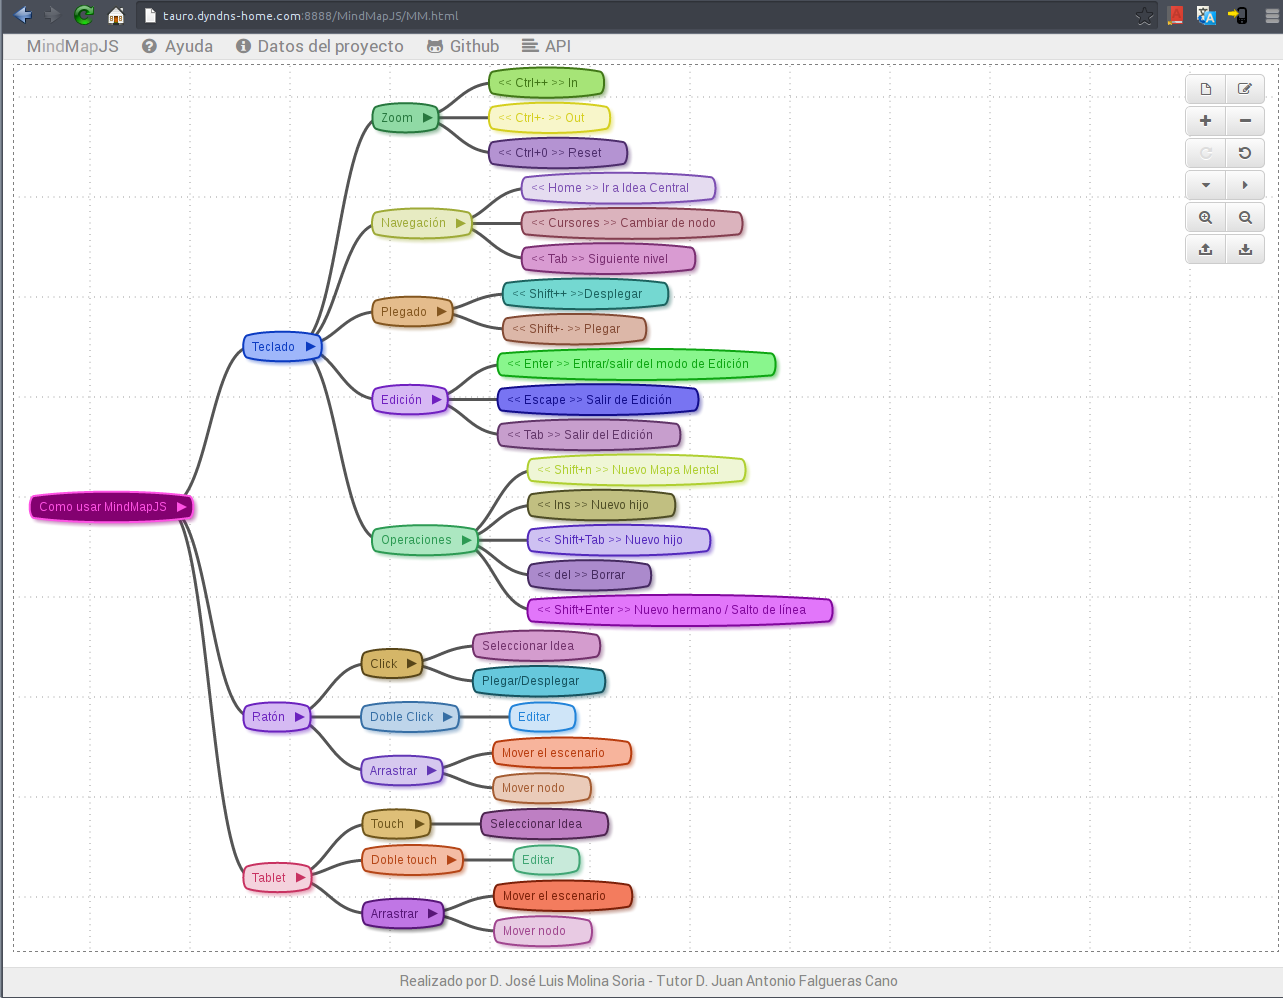
\includegraphics[width=\linewidth]{imagenes/MindMapJS1}
\caption{Página principal de MindMapJS}
\label{fig:MindMapJS}
\end{figure}


\subsection{Estructura de la página principal.}

En la página de inicio de MindMapJS (ver figura \ref{fig:MindMapJS}) podemos diferenciar claramente tres partes. 

\begin{itemize}
\item \textbf{Cabecera o menú superior.} En cual disponemos de algunos enlaces para despegar información sobre el proyecto (ver figura \ref{fig:Menu-datos-del-proyecto}).
\item \textbf{Pie.}
\item \textbf{Cuerpo.} Contenedor para el editor de mapas mentales.
\item \textbf{Barra de herramientas.} Con la funcionalidad básica para manejar interactuar con el Mapa mental.
\end{itemize}

\begin{figure}[tbph]
\centering
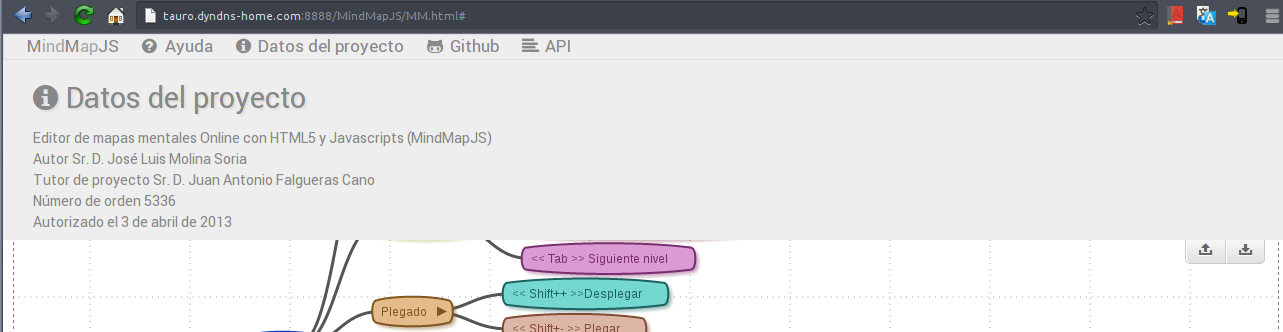
\includegraphics[width=\linewidth]{imagenes/MindMapJS2}
\caption{Menú > Datos del proyecto}
\label{fig:Menu-datos-del-proyecto}
\end{figure}

Al cargar la página (se puede ver en la figura \ref{fig:MindMapJS}) nos muestra un mapa mental con las formas de uso habituales. Mediante teclado, ratón o touch.

\subsection{Barra de herramientas.}

En la barra de herramientas disponemos de las siguientes opciones ( imagen \ref{fig:barra-herrramientas}), de izquierda a derecha y de arriba a bajo son:
\begin{itemize}
\item Nuevo: crea un nuevo mapa mental
\item Editar: establece el modo de edición para la idea activa.
\item Crear: crea una nueva idea.
\item Borrar: borra la idea activa.
\item Hacer: para volver a rehacer acciones deshechas. 
\item Deshacer: deshace la última acción realizada.
\item Plegar: pliega la subideas de la idea activa.
\item Desplegar: despliega una idea plegada.
\item Zoom in: amplia la escala del mapa mental.
\item Zoom out: reduce la escala del mapa mental.
\item Cargar: realiza la carga de un fichero freeMind.
\item Salvar: salva el mapa mental actual en un fichero freeMind.
\end{itemize}

\begin{figure}[tbph]
\centering
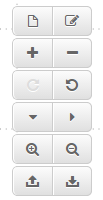
\includegraphics[width=0.1\linewidth]{imagenes/barraHerramientas}
\caption{Barra de herramientas}
\label{fig:barra-herrramientas}
\end{figure}


\subsection{¿Cómo crear un nuevo Mapa Mental?}
Para iniciar o crear un nuevo mapa mental podemos optar por hacer clic en el botón de la barra de herramientas, o bien pulsar la secuencia de teclas Shift+n. Una vez pulsado el botón para crear un nuevo mapa mental se borrará el mapa actual y preparará el editor para un nuevo mapa mental a partir de una nueva idea central (ver figura \ref{fig:MM-nuevo}).

\begin{figure}[tbph]
\centering
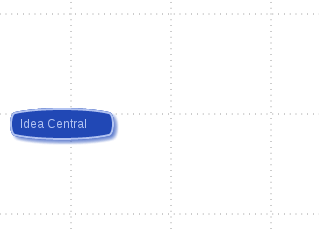
\includegraphics[width=0.4\linewidth]{imagenes/MM-nuevo.png}
\caption{Crear un nuevo mapa}
\label{fig:MM-nuevo}
\end{figure}


\subsection{Insertar nuevas subideas.}
Siempre podemos insertar una subidea a partir de otra ideal principal (ver figura \ref{fig:MM-insertar}) con el botón de la barra de herramientas, o pulsando la tecla ins. Siempre que generemos una nueva idea el editor pasara al modo de edición para que se pueda cambiar el contenido (ver figura \ref{fig:MM-edicion}). 

\begin{figure}[tbph]
\centering
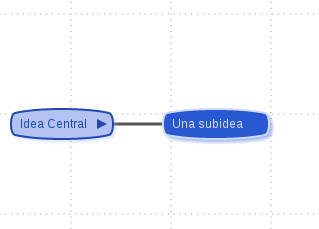
\includegraphics[width=0.4\linewidth]{imagenes/MM-insertar.png}
\caption{Inserción de subideas.}
\label{fig:MM-insertar}
\end{figure}

Si pulsamos Shift+Enter generaremos un idea hermana a la actual (ver figura \ref{fig:MM-insertar-hermana}), es decir, que depende de la misma idea principal. 

\begin{figure}[tbph]
\centering
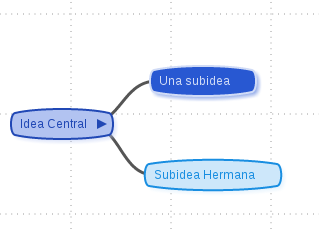
\includegraphics[width=0.4\linewidth]{imagenes/MM-insertar-hermana.png}
\caption{Inserción de subideas hermana.}
\label{fig:MM-insertar-hermana}
\end{figure}


\subsection{Editar idea.}

Para entrar en modo de edición de la idea actual podemos pulsar Enter, doble clic o pulsar el botón correspondiente en la barra de herramientas. Siempre podremos salir pulsando la tecla Escape, pulsando en otro punto de la pantalla con el ratón, o bien, volviendo a pulsar el botón de edición. 

\begin{figure}[tbph]
\centering
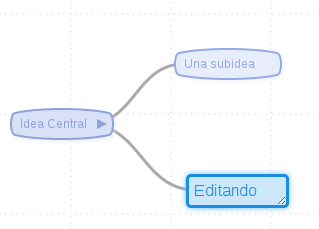
\includegraphics[width=0.4\linewidth]{imagenes/MM-edicion.png}
\caption{Editando una idea.}
\label{fig:MM-edicion}
\end{figure}


\subsection{Borrar idea.}
Una vez seleccionada la idea que deseamos borrar pulsaremos el botón de borrar o la tecla Supr. El proceso de borrado elimina todas las subideas de la idea borrada. 

\subsection{Navegar por el mapa.}
Como podrá observar siempre existe una idea seleccionada (tiene el cursor). Para poder movernos por las distintas ideas siempre podremos seleccionar una idea con el clic del ratón o tocando con el dedo en un dispositivo táctil. 

También disponemos de los cursores del teclado para desplazarnos por el mapa mental. La tecla home para ir a la idea principal y el tabulador para desplazarnos entre los distintos niveles.

\subsection{Plegar/desplegar.}

Por defecto, el editor MindMapJS, crear o muestra las ideas de forma desplegada ( como se puede ver en la siguiente figura \ref{fig:MM-desplegado} ). Si una idea tiene asociada una o más subideas, esta idea principal mostrará un pequeño triangulo como indicador des/plegado. Si el triangulo apunta hacia los hijos indica que la idea esta desplegada. Si el triangulo a punta hacia abajo indica que la idea esta plegada (ver imagen \ref{fig:MM-plegado}).  

\begin{figure}[tbph]
\centering
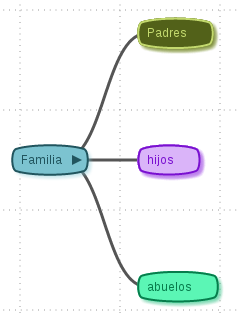
\includegraphics[width=0.3\linewidth]{imagenes/MM-desplegado.png}
\caption{Mapa mental desplegado.}
\label{fig:MM-desplegado}
\end{figure}

Para plegar o desplegar una idea, tan sólo debemos realizar un clic sobre el indicador de plegado (triangulo) o mediante el uso de la barra de herramienta. También se dispones de opciones de teclados Shift+- para plegar y Shift++ para desplegar. 

\begin{figure}[tbph]
\centering
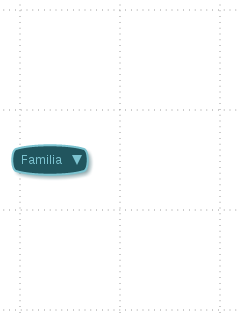
\includegraphics[width=0.3\linewidth]{imagenes/MM-plegado.png}
\caption{Mapa mental plegado.}
\label{fig:MM-plegado}
\end{figure}


\subsection{Zoom. Ampliar y reducir la imagen.}

Para ampliar o reducir el mapa mental como siempre disponemos de distintas opciones. 

\begin{figure}[tbph]
\centering
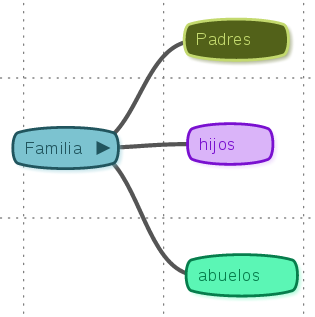
\includegraphics[width=0.3\linewidth]{imagenes/MM-zoom-in.png}
\caption{Mapa mental con ampliado.}
\label{fig:MM-zoom-in}
\end{figure}

Se puede utilizar los botones de la barra de herramientas (icono de la lupa). La secuencias de teclas: Ctrl++ para ampliar (imagen \ref{fig:MM-zoom-out}); Ctrl+- para reducir (imagen \ref{fig:MM-zoom-in}) y Ctrl+0 para reiniciar la escala de la imagen.  

\begin{figure}[tbph]
\centering
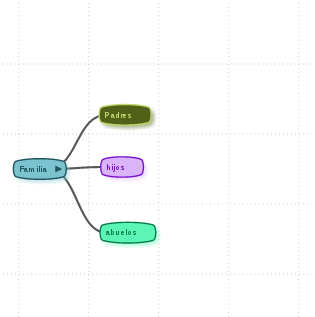
\includegraphics[width=0.3\linewidth]{imagenes/MM-zoom-out.png}
\caption{Mapa mental con reducido.}
\label{fig:MM-zoom-out}
\end{figure}

También dispones de la rueda de ratón para cambiar el tamaño o escala de nuestro mapa mental. 

\subsection{Listado de secuencias de teclado. Keystrokes.}

\begin{tabular}{|c|c|}
	\hline
	\textbf{Secuencia de teclado} &                \textbf{Acción}                \\ \hline
	           Ctrl++             &                    Zoom in                    \\ \hline
	           Ctrl+-             &                   Zoom out                    \\ \hline
	           Ctrl+0             &               Resetear el zoom                \\ \hline
	            home              &               Ir a idea central               \\ \hline
	          cursores            &  Para moverse por las ideas del mapa mental   \\ \hline
	             Tab              &   Para moverse al siguiente nivel del mapa    \\ \hline
	             Tab              &  Crear nueva idea si no hay siguiente nivel.  \\ \hline
	             Tab              &          Desplegar un nodo plegado.           \\ \hline
	            Enter             &     Pone la idea actual en modo edición.      \\ \hline
	           Escape             &           Sale del modo de edición.           \\ \hline
	           Shift++            &          Desplegar un nodo plegado.           \\ \hline
	           Shift+-            &            Plegar un nodo plegado.            \\ \hline
	           Shift+n            &              Nuevo mapa mental.               \\ \hline
	             ins              &               Nueva idea hija.                \\ \hline
	          Shift+Tab           &               Nueva idea hija.                \\ \hline
	             del              &             Borra la idea actual.             \\ \hline
	         Shift+Enter          &         Crea una nueva idea hermana.          \\ \hline
	         Shift+Enter          & Inserta un salto de línea en modo de edición. \\ \hline
\end{tabular} 
